\chapter{時系列CSI予測モデル更新のための補間手法比較}{}
\label{chap:4th}

\section{はじめに}
本章では,前章までで述べた時系列CSI予測の環境適応に関する研究を踏まえ,実運用の視点から問題点を整理する.
その上で,本研究で対象とする課題を明確化し,実験結果を示す.

\section{はじめに}
\label{sec:related_work_and_problems}
前章で述べた時系列CSI予測の環境適応に関する研究について,少量データでの適応を狙うメタ学習に基づく初期化学習\cite{kim2023_meta_denoising_mimo},事前学習済みモデルとして大規模言語モデルを転用する研究\cite{liu2024_llm4cp},運用中の分布変化に逐次追従する継続学習\cite{mohsin2025_continual_learning_channel_prediction}などがあった.

既存研究の多くは,新環境で得られる正解データを用いたモデル更新を前提としている.一方,CSI予測で参照信号を削減する場合,予測スロットでは参照信号を送らないため,予測対象時刻のCSI推定値が得られない.このとき,時系列CSI予測モデルの正解ラベルfを獲得できないため,教師あり学習に基づく損失を計算できず,予測を継続しながら逐次的にモデルを更新することが難しい.

具体例として,時刻\(t\)のCSI推定値を\(\bm{H}_t\),予測値を\(\widehat{\bm{H}}_t\)とする.3入力1出力の予測モデルを運用する場合,\(\bm{H}_t,\bm{H}_{t+1},\bm{H}_{t+2}\)から\(\widehat{\bm{H}}_{t+3}\)を得る.参照信号を削減する予測スロットでは,時刻\(t+3\)の推定値\(\bm{H}_{t+3}\)を獲得できない.その結果,\(\widehat{\bm{H}}_{t+3}\)に対する教師信号が欠落し,更新用の学習データを逐次獲得することができない.

このとき,運用で基地局が利用できるCSI系列は,推定値と予測値が混在する系列となる.上の例では,時刻\(t\)から\(t+3\)にかけて\(\bm{H}_t,\bm{H}_{t+1},\bm{H}_{t+2},\widehat{\bm{H}}_{t+3}\)が得られる一方で,\(\bm{H}_{t+3}\)は欠落する.この混在系列を用いてモデルを更新する方法として,三つの方針が考えられる.

第1に,一時的に予測を停止し,参照信号を送信して全時刻の推定値を揃えた後に更新する方針である.しかし,参照信号削減という時系列CSI予測の目的に反するうえ,更新までの遅延も増大する.
加えて,運用中にモデルを停止する場合,停止と再開の手順,許容中断時間,それに伴う遅延を考慮した運用方針を設計する必要がある.しかし,これらに関する標準化は検討途上であり,具体的要件は十分に整理されていないため,実装上の困難が伴う.
移動通信システムの仕様を策定する国際標準化プロジェクトである3GPPでは無線機能に関する要件を扱う立場からAIと機械学習の適用に伴う要件を議論している\cite{3gpp_tr38843}.具体的には,AIモデルの配布,導入,有効化,無効化,切り替え,更新などの運用手順を含むライフサイクル管理と,これらの手順に伴う遅延と中断に関する要件である\cite{3gpp_tr38843}.商用展開に向けてモデル汎化,モデル切り替え,モデル更新の三つのアプローチが調査されているが,モデル有効化と無効化,切り替え時の遅延の扱いは議論中であり,具体的な規定は策定途上にある\cite{nokia_aiml_ran}.
また,モデル切り替え時に推論をどのモデルが担うか,切り替え中の推論の中断をどの程度許容するか,切り替え判断の基準をどのように定めるかなど基本的事項が未解決であり,Release 19以降の検討に委ねられている\cite{arxiv_3gpp_standardization}.
3GPPでの標準化検討とは別に,産業界ではAI-RANとして,無線アクセスネットワークにAIモデルを組み込み,時系列CSI予測のような推論をRAN機能の近傍でリアルタイムに実行する次世代アーキテクチャが議論されている\cite{wia_challenges}.リアルタイム推論の実行には低遅延のエッジインフラや限られた計算資源で動作する軽量モデルに加え,AIモデルの障害時にRANが機能を維持するためのフォールバック機構が求められる\cite{wia_challenges}.一方で,フォールバック機構の設計指針は確立されておらず,推論を一時停止してレガシー手順へ切り替える際の中断時間やサービス品質への影響を制御する標準的な枠組みは存在しない.
以上より,予測停止に基づく第1の方針は参照信号削減の利点を損なうだけでなく,実運用における実現可能性にも課題を残す.

第2に,予測対象時刻を正解ラベルとみなし,\(\widehat{\bm{H}}_{t+3}\)に対して時刻\(t+3\)の正解を与えて更新する方針である.しかし,参照信号削減下では\(\bm{H}_{t+3}\)を獲得できないため,予測値との間の損失計算が成り立たず,教師あり学習ができない.
他分野では,観測や正解データが継続的に得られるため,データの到着に合わせて逐次更新する枠組みが一般的である.気象予測では観測値を取り込み,データ同化により状態推定と予報を反復する\cite{kalnay2003_atmospheric_modeling,evensen2003_enkf}.金融予測では市場価格やリターンが逐次観測され,オンライン学習により予測モデルを更新する\cite{cover1991_universal_portfolios}.データ分布が時間とともに変化する問題設定は概念ドリフトとして整理され,適応手法が議論されている\cite{gama2014_concept_drift_survey}.
しかし,時系列CSI予測の分野では,予測スロットでは参照信号を送らないため,予測対象時刻のCSI推定値が得られない.


第3に,入力に予測値を含め,次に推定値が得られる時刻を正解ラベルとして更新する方針である.例えば\(\bm{H}_{t+1},\bm{H}_{t+2},\widehat{\bm{H}}_{t+3}\)から\(\bm{H}_{t+4}\)を学習する.
ただし,入力に予測誤差が混入し,誤差蓄積による性能劣化を招く可能性が指摘されている\cite{jiang2022_transformer_mobility_negligible}.

以上より,参照信号削減を前提とする時系列CSI予測の運用では,推定値と予測値が混在するCSI系列から,予測を継続しながらモデルを更新する枠組みが必要となる.前節で述べた第1の方針は参照信号削減の目的と整合しないだけでなく,停止と再開に伴う運用手順や遅延と中断に関する要件が標準化検討途上である点からも,実装上の負担が大きい.そのため本研究では,第2および第3の方針が想定する状況,すなわち予測を継続したまま欠損する正解ラベルを扱いながら更新する問題を対象とする.




\subsection{提案機構の概要}
本研究では,参照信号削減のため予測スロットでは参照信号を送信せず,そのスロットのCSI推定値が得られない状況を前提として,予測を継続したまま時系列CSI予測モデルを更新する枠組みを提案する.
本枠組みの要点は,予測スロットで欠損する教師信号,すなわち正解ラベルに対し,後続スロットで観測されるCSI推定値に基づき補間値を算出し,更新用データを生成する点にある.
提案機構の概要を図\ref{fig:explonation}に示す.

以下,時刻\(t\)をスロット時刻とし,参照信号から得るCSI推定値を\(\bm{H}_t\),予測モデルが出力するCSI予測値を\(\widehat{\bm{H}}_t\)とする.
補間により得られる予測スロットの補間値を\(\widetilde{\bm{H}}_t\)とする.
説明のため,直近3スロットを入力として1スロット先を予測する3入力1出力の予測モデルを例にとる.このとき,学習済み予測モデル\(f_{\theta}\)により
\begin{equation}
  \widehat{\bm{H}}_{t+3}=f_{\theta}(\bm{H}_t,\bm{H}_{t+1},\bm{H}_{t+2})
\end{equation}
を得る.しかし,参照信号削減の運用では予測スロット\(t+3\)において参照信号を送信しないため,\(\bm{H}_{t+3}\)は観測できず,\(\widehat{\bm{H}}_{t+3}\)に対する教師信号が欠落する.

そこで本研究では,予測スロットより後に得られる推定値を用い,欠損した\(\bm{H}_{t+3}\)を事後的に推定する.
具体的には,次スロット以降で参照信号が送信されて\(\bm{H}_{t+4},\bm{H}_{t+5},\dots\)が得られたら,欠損時刻の前後に存在する推定値を用いて補間し,予測スロットに対応する補間値
\begin{equation}
  \widetilde{\bm{H}}_{t+3}
\end{equation}
を算出する.この\(\widetilde{\bm{H}}_{t+3}\)は,予測スロットで本来得られるべき\(\bm{H}_{t+3}\)の近似として扱うことで,教師あり学習に必要な正解ラベルを近似的に回復する役割を担う.

補間値が得られた後は,逐次得られる推定値と組み合わせて更新用の学習サンプルを構成し,予測モデルをファインチューニングする.
例えば,入力を\(\widetilde{\bm{H}}_{t+3},\bm{H}_{t+4},\bm{H}_{t+5}\),出力を\(\bm{H}_{t+6}\)として学習サンプルを作成し,これを用いてモデルを更新する.
ここで,3入力の並びは一例であり,入力の3時刻のうち予測スロットに対応する1点を\(\widetilde{\bm{H}}\)で置き換え,残りを後続スロットで得られる推定値で構成すればよい.
すなわち,
\begin{equation}
  \bm{H}_{t+6}\approx f_{\theta}(\widetilde{\bm{H}}_{t+3},\bm{H}_{t+4},\bm{H}_{t+5})
\end{equation}
となるように損失を計算し,勾配法によりモデルを微調整する.

以上の手順を繰り返すことで,参照信号削減下でも予測スロットにおける欠損ラベルを補間により補いながら,予測処理を中断せずに運用データから更新用サンプルを逐次生成できる.
これにより,環境変化に伴う分布の変化に追従したモデル更新を実現する.




\begin{figure}[H]
  \centering
  \includegraphics[width=120mm]{../picture/4nd/explonation_pdf15.pdf}
  \caption{提案機構の概要}
  \label{fig:explonation}
\end{figure}



\subsubsection{補間手法}
\label{sec:interpolation_methods}
本節では,本論文で用いる補間手法を説明する.本研究の枠組みでは,予測スロットにおいて\(\bm{H}_t\)が欠損するため,後続スロットで得られる推定値から補間値\(\widetilde{\bm{H}}_t\)を算出し,更新用サンプルの入力に用いる.
補間は時間方向に対して行い,各スロットのCSIをフラット化した特徴量ベクトルの各次元に対して,同一の補間手順を適用する.
本論文では,複数の補間手法を比較対象として用いる.以下に示す補間手順は実装の一例であり,補間対象時刻の前後に存在する推定値から\(\widetilde{\bm{H}}_t\)を得るという点が共通である.
補間対象時刻より後に得られる推定値も用いるため,欠損を一方向の外挿として扱う場合に比べて,補間値の推定誤差を抑えられる.

\subsubsection{線形補完}
最も簡単な基準手法として,補間対象時刻の前後1スロットで得られる推定値の平均を補間値とする.
補間対象時刻を\(t\)とすると,\(\bm{H}_{t-1}\)と\(\bm{H}_{t+1}\)から補間値\(\widetilde{\bm{H}}_t\)を
\begin{equation}
  \widetilde{\bm{H}}_t=\frac{1}{2}\left(\bm{H}_{t-1}+\bm{H}_{t+1}\right)
\end{equation}
として算出する.

\subsubsection{スプライン補間}
スプライン補間では,補間対象時刻の前後に存在する複数スロットの推定値を用い,時間方向に平滑な曲線で\(\widetilde{\bm{H}}_t\)を算出する.
具体例として,補間対象を\(\bm{H}_3\)とし,近傍として\(\bm{H}_0,\bm{H}_1,\bm{H}_2,\bm{H}_4,\bm{H}_5,\bm{H}_6\)の6点を用いる.
補間対象時刻\(t=3\)からの相対時刻を\(\tau\)とし,\(\tau\)が取り得る値の集合を\(\mathcal{T}=\{-3,-2,-1,1,2,3\}\)と定義する.
すなわち,\(\tau=-3\)は時刻0,\(\tau=1\)は時刻4に対応する.このとき,観測点を
\begin{equation}
  \left\{(\tau,\bm{H}_{3+\tau})\mid \tau\in\mathcal{T}\right\}
\end{equation}
と表す.この観測点を通過する三次スプライン関数\(\bm{s}(\tau)\)を構成し,
\begin{equation}
  \bm{s}(\tau)=\bm{H}_{3+\tau}\quad \tau\in\mathcal{T}
\end{equation}

を満たすように係数を定める.境界条件は自然スプラインとする.これは,観測区間の両端で曲率が0となる条件を課し,端点付近で過度に曲がることを抑える設定である.\(\tau=0\)で評価して

\begin{equation}
  \widetilde{\bm{H}}_3=\bm{s}(0)
\end{equation}
を得る.


\subsubsection{低次多項式近似}
多項式近似では,時間方向のみに対して低次多項式を当てはめ,補間対象時刻の値を推定して\(\widetilde{\bm{H}}_t\)を算出する.
補間対象を時刻\(t\)とし,補間対象時刻からの相対時刻を\(\tau\)とする.近傍として用いる\(\tau\)の集合を\(\mathcal{T}=\{\tau_1,\ldots,\tau_K\}\)とする.
このとき,\(\tau_i\in\mathcal{T}\)に対応する観測値を\(\bm{H}_{t+\tau_i}\)とし,次数\(d\)の多項式
\begin{equation}
  \bm{p}(\tau)=\sum_{m=0}^{d}\bm{a}_m \tau^m
\end{equation}
により時間方向の変化を近似する.係数\(\{\bm{a}_m\}_{m=0}^{d}\)は最小二乗により
\begin{equation}
  \{\bm{a}_m\}=\arg\min_{\{\bm{a}_m\}}\sum_{i=1}^{K}\left\lVert \bm{H}_{t+\tau_i}-\bm{p}(\tau_i)\right\rVert_2^2
\end{equation}
として推定する.推定後,\(\tau=0\)で評価して補間値を
\begin{equation}
  \widetilde{\bm{H}}_t=\bm{p}(0)=\bm{a}_0
\end{equation}
として得る.

本論文では,多項式の次数\(d\)と近傍点数\(K\)を変化させ,補間精度と更新後の予測精度の関係を比較する.
次数の比較では,\(\mathcal{T}=\{-3,-2,-1,1,2,3\}\)の6点を用い,\(d\in\{2,3,4\}\)を比較する.
近傍点数の比較では,参照信号削減に伴う欠測の周期を\(P=4\)とし,欠測時刻に対応する時刻差を近傍候補から除外する.
具体的には,\(\mathbb{Z}\)を整数集合として,候補集合を
\begin{equation}
  \mathcal{C}=\{\tau\in\mathbb{Z}\mid \tau\neq 0,\ \tau\not\equiv 0\ (\mathrm{mod}\ P)\}
\end{equation}
と定義し,\(\mathcal{C}\)から負の側に\(k_{\mathrm{true}}\)点,正の側に\(k_{\mathrm{true}}\)点を近い順に選び,
\begin{equation}
  \mathcal{T}=\{\tau\in\mathcal{C}\mid \tau<0\}^{k_{\mathrm{true}}}\cup \{\tau\in\mathcal{C}\mid \tau>0\}^{k_{\mathrm{true}}}
\end{equation}
として近傍点集合を構成する.ここで,\(\{\cdot\}^{k_{\mathrm{true}}}\)は絶対値が小さい順に\(k_{\mathrm{true}}\)点を選ぶ演算を表す.
例として,\(k_{\mathrm{true}}=3\)では\(\mathcal{T}=\{-3,-2,-1,1,2,3\}\)となり,\(k_{\mathrm{true}}\)を増やすことで\(\pm 4,\pm 8,\ldots\)を除外しつつ,より遠方の真値点を近傍に含める.

\subsubsection{ニューラルネットワークを用いた補間}
ニューラルネットワークを用いた補間では,補間対象時刻を\(t\)とし,補間に用いる時刻差の集合\(\mathcal{T}=\{-3,-2,-1,1,2,3\}\)に対応する推定値を入力として,\(\bm{H}_t\)への回帰を学習する.
\(\bm{H}_{t+\tau}\)をフラット化したベクトルを\(\bm{h}_{t+\tau}\)とし,入力ベクトルを
\begin{equation}
  \bm{x}_t=\left[\bm{h}_{t-3}^{\mathsf{T}},\bm{h}_{t-2}^{\mathsf{T}},\bm{h}_{t-1}^{\mathsf{T}},\bm{h}_{t+1}^{\mathsf{T}},\bm{h}_{t+2}^{\mathsf{T}},\bm{h}_{t+3}^{\mathsf{T}}\right]^{\mathsf{T}}
\end{equation}
と定義する.サンプルごとの振幅差を抑えるため,\(\bm{x}_t\)をRMSで正規化し,
\begin{equation}
  \alpha_t=\sqrt{\frac{1}{\mathrm{dim}(\bm{x}_t)}\left\lVert \bm{x}_t\right\rVert_2^2},\quad
  \bar{\bm{x}}_t=\frac{1}{\alpha_t}\bm{x}_t
\end{equation}
を得る.学習済み補間器を\(g_{\phi}(\cdot)\)とする.ここで,\(g_{\phi}\)の出力は補間対象時刻のCSIをフラット化したベクトルであり,\(\widetilde{\bm{h}}_t\)と表す.補間値は
\begin{equation}
  \widetilde{\bm{h}}_t=\alpha_t\, g_{\phi}(\bar{\bm{x}}_t)
\end{equation}
として算出する.\(\widetilde{\bm{h}}_t\)をスロット\(t\)のCSI行列の形状に戻すことで\(\widetilde{\bm{H}}_t\)を得る.



\subsection{モデルのアーキテクチャ}
本論文で用いるニューラルネットワークのアーキテクチャについて説明する.
本論文では時系列CSI予測を実行するニューラルネットワークと補間を実行するニューラルネットワークの2種類がある。

\subsubsection{予測ニューラルネットワーク}

本論文のCSI予測器(CSI Predictor)は,全結合層からなる多層パーセプトロン(MLP)として実装する(`scripts/model.py` の `class MLP`).
時刻方向に過去\(T_I\)フレーム分のCSIを用い,各フレームをベクトル化して結合した入力\(\bm{x}\in\mathbb{R}^{T_I\cdot F}\)から,次フレーム1枚分のCSIをベクトル化した出力\(\widehat{\bm{y}}\in\mathbb{R}^{F}\)を回帰する.
ここで,\(F\)は1フレームのCSI(行列)をフラット化した次元である.

inside-cellの実験ログにおける具体例として,\(T_I=3\),\(F=3072\)のとき,入力次元は\(\mathrm{in\_dim}=T_I\cdot F=9216\),出力次元は\(\mathrm{out\_dim}=F=3072\)となる.

MLPの層構成(デフォルト設定)は以下のとおりである.中間層ではReLUにより非線形性を導入し,過学習を抑制するためにDropout(\(p=0.1\))を適用する.
\begin{itemize}
  \item \(\mathrm{Linear}(\mathrm{in\_dim}\rightarrow 2048)\rightarrow \mathrm{ReLU}\rightarrow \mathrm{Dropout}(p=0.1)\)
  \item \(\mathrm{Linear}(2048\rightarrow 1024)\rightarrow \mathrm{ReLU}\rightarrow \mathrm{Dropout}(p=0.1)\)
  \item \(\mathrm{Linear}(1024\rightarrow 512)\rightarrow \mathrm{ReLU}\rightarrow \mathrm{Dropout}(p=0.1)\)
  \item \(\mathrm{Linear}(512\rightarrow \mathrm{out\_dim})\)
\end{itemize}
以上により,過去\(T_I\)フレームに含まれる時系列情報を,固定長ベクトル\(\bm{x}\)として受け取り,次フレームのCSIベクトル\(\widehat{\bm{y}}\)を直接推定する.


\subsubsection{補間ニューラルネットワーク}

補間器は,欠損している中心時刻\(t\)のCSI \(\bm{H}_t\)を,その前後の近傍フレームから推定するニューラルネットワークである.
本論文では,context\_size\(=3\)として\(\mathcal{T}=\{-3,-2,-1,1,2,3\}\)の6近傍フレームを用い,それらをフラット化して結合した入力\(\bm{x}_t\in\mathbb{R}^{6F}\)から,中心フレーム1枚分のCSIをフラット化した出力\(\widetilde{\bm{h}}_t\in\mathbb{R}^{F}\)を推定する.
得られた\(\widetilde{\bm{h}}_t\)を行列形状に戻すことで補間値 \(\widetilde{\bm{H}}_t\)を構成する.

\paragraph{MLP補間器}
基本設定の補間器は,全結合層からなるMLPとして実装する.context\_size\(=3\)のときの層構成は以下のとおりである(活性化はReLU).
\begin{itemize}
  \item \(\mathrm{Linear}(6F\rightarrow 2048)\rightarrow \mathrm{ReLU}\)
  \item \(\mathrm{Linear}(2048\rightarrow 1024)\rightarrow \mathrm{ReLU}\)
  \item \(\mathrm{Linear}(1024\rightarrow F)\)
\end{itemize}

\paragraph{RMS正規化(学習・推論で共通)}
チャネル全体のスケール変動に対して学習を安定化させるため,入力\(\bm{x}_t\)のRMSから正規化係数\(\alpha_t\)を計算し,\(\bar{\bm{x}}_t=\bm{x}_t/\alpha_t\)を補間器へ入力する(式(\ref{tab:training_hyperparams})より前で定義した\(\alpha_t\)および\(\bar{\bm{x}}_t\)と同一).
補間器の出力は元スケールへ戻して用い,\(\widetilde{\bm{h}}_t=\alpha_t\,g_{\phi}(\bar{\bm{x}}_t)\)として\(\widetilde{\bm{H}}_t\)を得る.

\paragraph{3D CNN補間器(オプション)}
補間器の選択肢として,3次元畳み込みニューラルネットワーク `InterpolatorCNN3D` も用意する.
設定 `--interpolator-model cnn3d` のときに利用され,context\_size\(=3\)(前後3フレームの計6フレーム)に固定される.
このモデルは,入力CSIをフラット化せずテンソルとして扱い,時間方向(近傍フレーム)と周波数・アンテナ方向の局所相関を3D畳み込みにより抽出して,中心フレームのCSIを回帰する設計である.

\begin{table}[H]
  \centering
  \caption{学習で用いたハイパーパラメータ}
  \label{tab:training_hyperparams}
  \begin{tabular}{lccc}
    \hline
    フェーズ & エポック数 & バッチサイズ & 学習率 \\
    \hline
    予測モデル学習 & 40 & 256 & $10^{-3}$ \\
    補間モデル学習 & 10 & 128 & $10^{-4}$ \\
    予測モデルファインチューニング & 20 & 128 & $10^{-4}$ \\
    \hline
  \end{tabular}
\end{table}


\subsubsection{学習とテスト}



\subsubsection{評価指標}
本論文の評価指標には,正規化平均二乗誤差 Normalized Mean Squared Error,NMSEを用いる.
NMSEは,推定値と真値の二乗誤差を真値の電力で正規化した量であり,サンプルごとに算出した後に平均する.

本論文では,補間の精度を表す補間NMSEと,予測モデルの精度を表す予測NMSEを区別して評価する.

\paragraph{補間NMSE}
補間NMSEは,補間器が出力する補間値\(\widetilde{\bm{H}}_t\)と,欠損していた真値\(\bm{H}_t\)の誤差を評価する.
\begin{equation}
  \mathrm{NMSE}_{\mathrm{interp}}
  =\frac{\left\lVert \widetilde{\bm{H}}_t-\bm{H}_t\right\rVert_2^2}{\left\lVert \bm{H}_t\right\rVert_2^2}
  \label{eq:nmse_interp_def}
\end{equation}

\paragraph{予測NMSE}
予測NMSEは,予測モデルが出力する予測値\(\widehat{\bm{H}}_t\)と真値\(\bm{H}_t\)の誤差を評価する.
\begin{equation}
  \mathrm{NMSE}_{\mathrm{pred}}
  =\frac{\left\lVert \widehat{\bm{H}}_t-\bm{H}_t\right\rVert_2^2}{\left\lVert \bm{H}_t\right\rVert_2^2}
  \label{eq:nmse_pred_def}
\end{equation}


\subsection{学習・評価データセットを生成するシミュレーション}

Sionna\cite{Makhlouf2025MOCSID}のレイトレーシングにより生成したCSI系列を用いてシミュレーション評価を行う.
OpenStreetMapから取得した地形データを三次元モデル化し,Sionnaへ入力してCSI系列を生成する.

\begin{table}[H]
  \centering
  \caption{三次元モデル化に用いたエリア}
  \label{tab:modeled_areas}
  \begin{tabular}{lll}
    \hline
    エリア & 中心座標 & 位置の目安 \\
    \hline
    新宿 & \(35.693^\circ\mathrm{N}, 139.703^\circ\mathrm{E}\) & 新宿区役所前交差点付近 \\
    池袋 & \(35.729^\circ\mathrm{N}, 139.713^\circ\mathrm{E}\) & 池袋駅東口前の明治通り付近 \\
    渋谷 & \(35.659^\circ\mathrm{N}, 139.700^\circ\mathrm{E}\) & 道玄坂下交差点付近 \\
    錦糸町 & \(35.6958^\circ\mathrm{N}, 139.8145^\circ\mathrm{E}\) & 錦糸町駅前交差点付近 \\
    \hline
  \end{tabular}
\end{table}


\begin{figure}[H]
  \centering
  \begin{subfigure}{0.49\textwidth}
    \centering
    \includegraphics[width=\textwidth]{../picture/4nd/ikebukuro_1.png}
    \caption{池袋(詳細1)}
    \label{fig:ikebukuro_1}
  \end{subfigure}
  \hfill
  \begin{subfigure}{0.49\textwidth}
    \centering
    \includegraphics[width=\textwidth]{../picture/4nd/ikebukuro_2.png}
    \caption{池袋(詳細2)}
    \label{fig:ikebukuro_2}
  \end{subfigure}

  \vspace{2mm}
  \begin{subfigure}{0.8\textwidth}
    \centering
    \includegraphics[width=\textwidth]{../picture/4nd/ikebukuro_fukan.png}
    \caption{池袋(俯瞰)}
    \label{fig:ikebukuro_fukan}
  \end{subfigure}
  \caption{三次元モデル化に用いたエリア(池袋)}
  \label{fig:area_ikebukuro}
\end{figure}

\begin{figure}[H]
  \centering
  \begin{subfigure}{0.49\textwidth}
    \centering
    \includegraphics[width=\textwidth]{../picture/4nd/shibuya_1.png}
    \caption{渋谷(詳細1)}
    \label{fig:shibuya_1}
  \end{subfigure}
  \hfill
  \begin{subfigure}{0.49\textwidth}
    \centering
    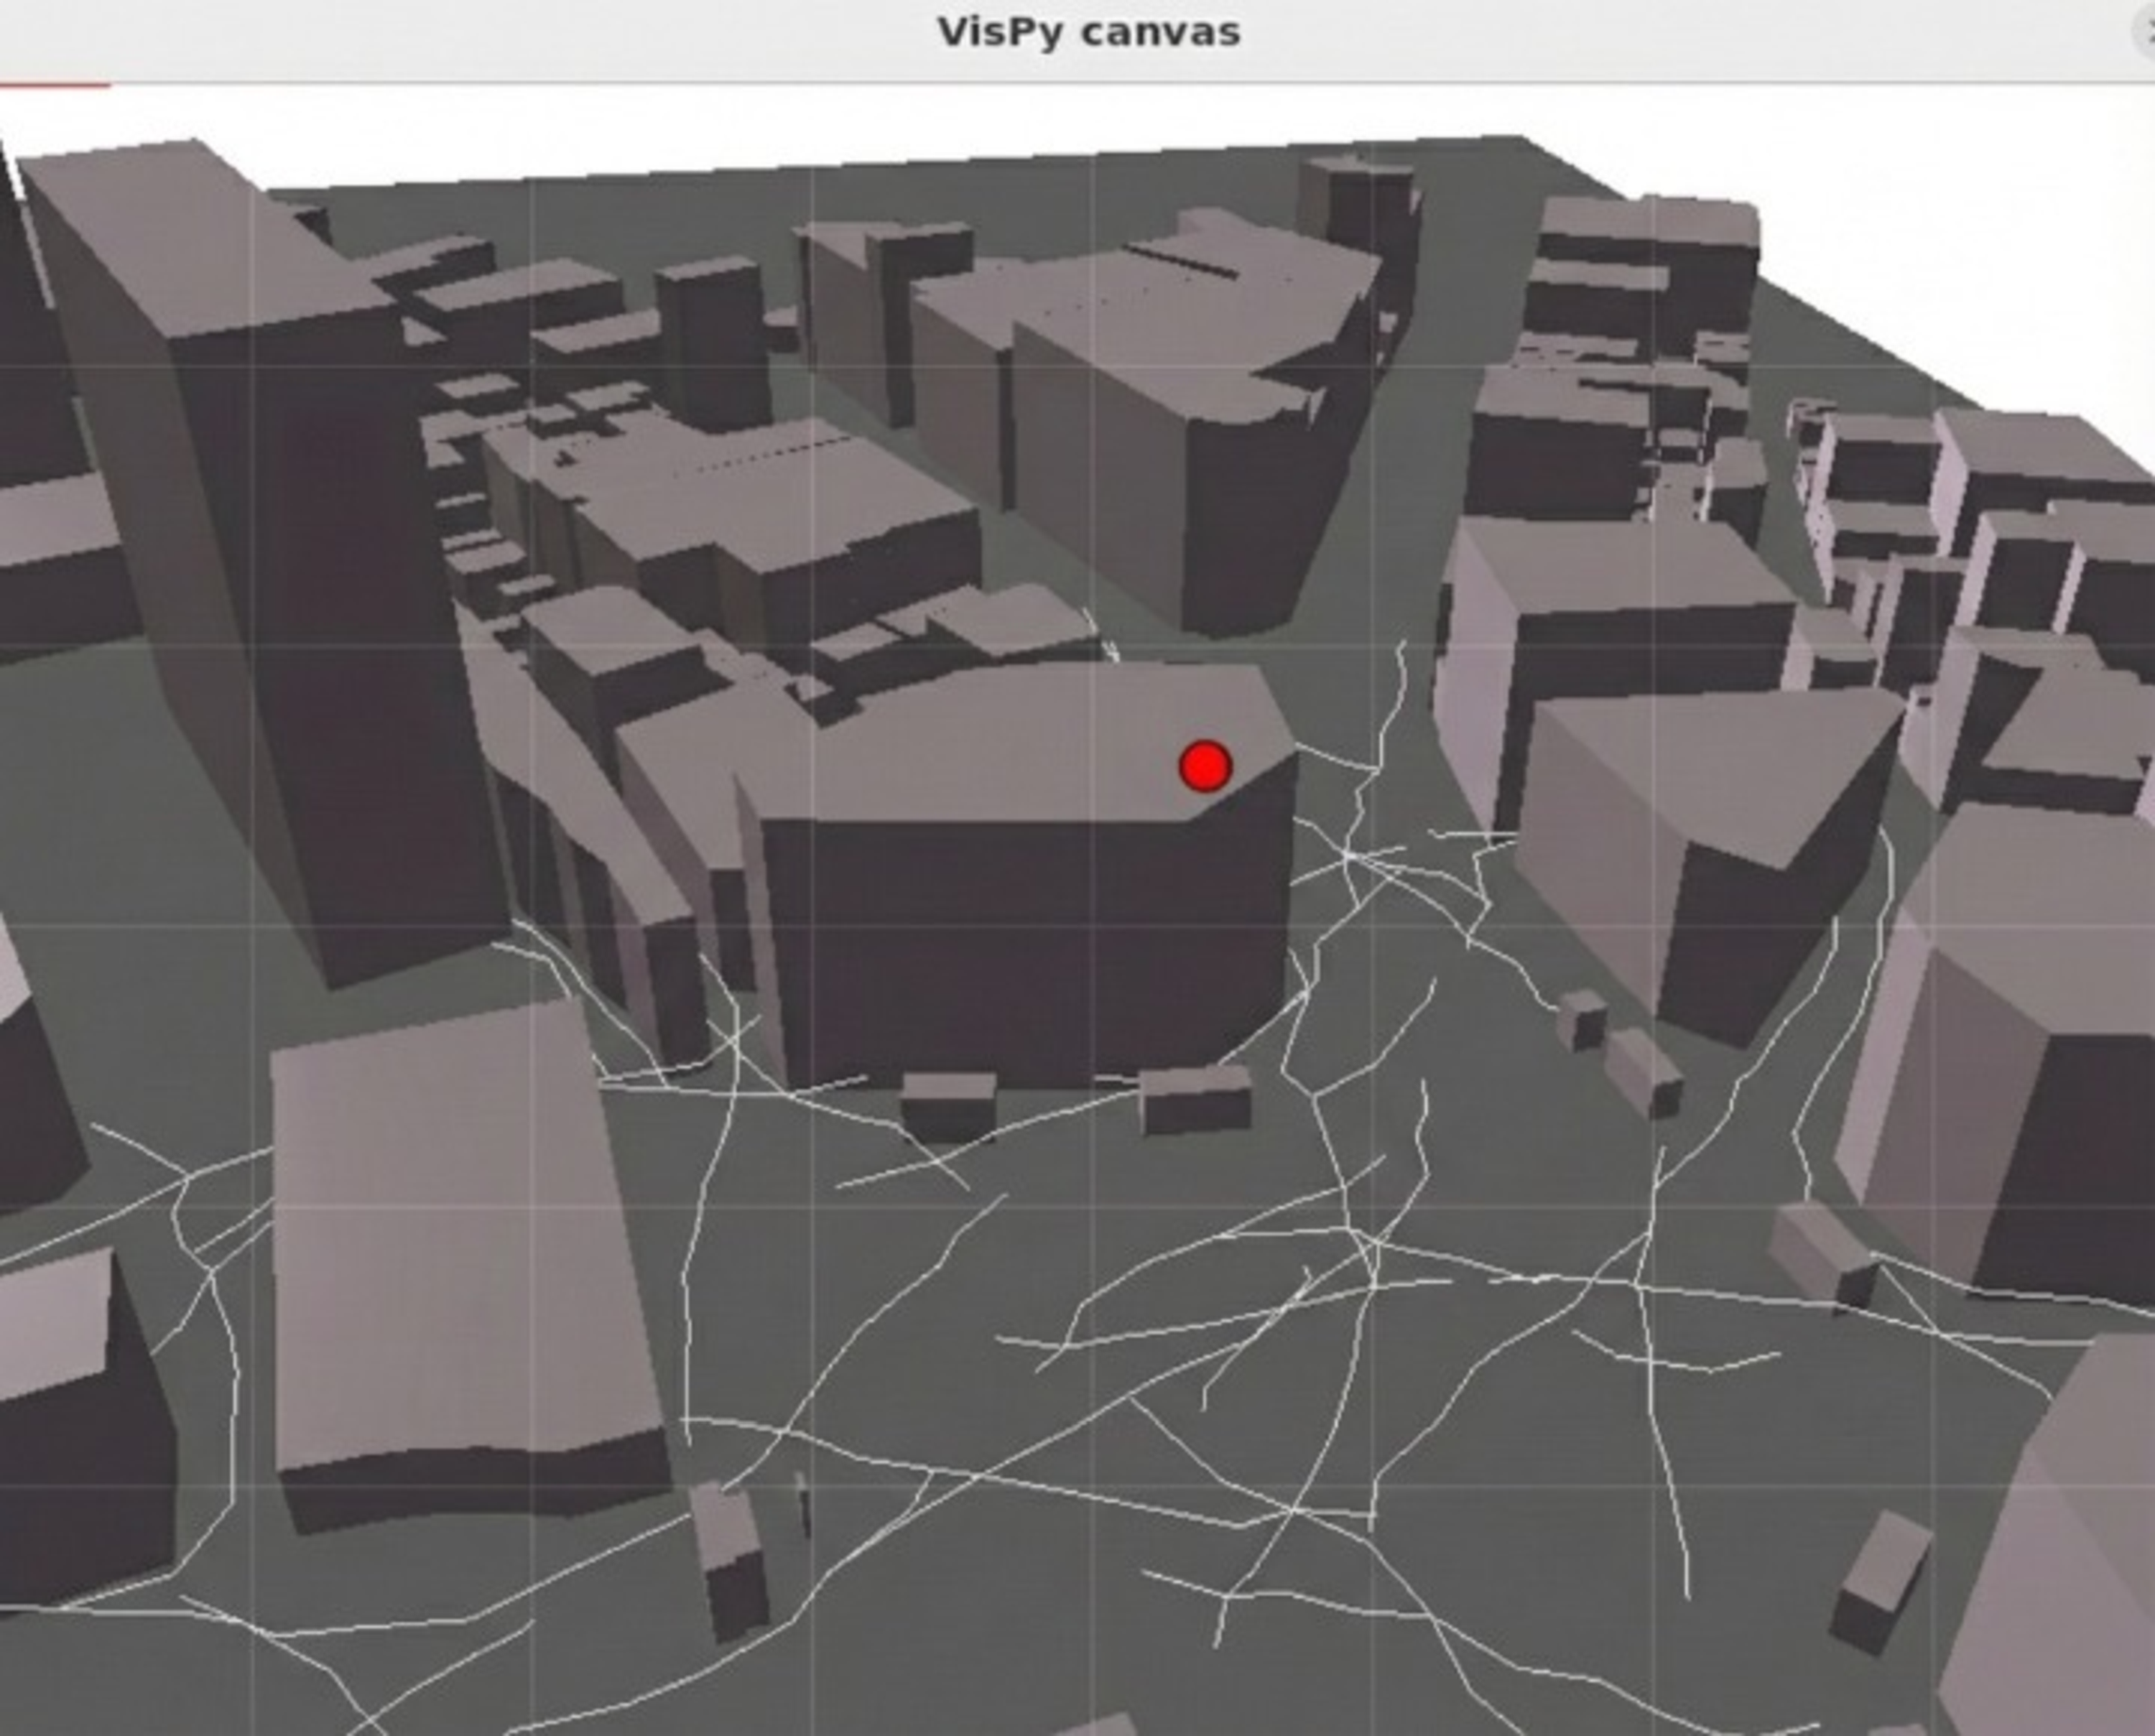
\includegraphics[width=\textwidth]{../picture/4nd/shibuya_2.png}
    \caption{渋谷(詳細2)}
    \label{fig:shibuya_2}
  \end{subfigure}

  \vspace{2mm}
  \begin{subfigure}{0.8\textwidth}
    \centering
    \includegraphics[width=\textwidth]{../picture/4nd/shibuya_fukan.png}
    \caption{渋谷(俯瞰)}
    \label{fig:shibuya_fukan}
  \end{subfigure}
  \caption{三次元モデル化に用いたエリア(渋谷)}
  \label{fig:area_shibuya}
\end{figure}

\begin{figure}[H]
  \centering
  \begin{subfigure}{0.49\textwidth}
    \centering
    \includegraphics[width=\textwidth]{../picture/4nd/shinjuku_1.png}
    \caption{新宿(詳細1)}
    \label{fig:shinjuku_1}
  \end{subfigure}
  \hfill
  \begin{subfigure}{0.49\textwidth}
    \centering
    \includegraphics[width=\textwidth]{../picture/4nd/shinjuku_2.png}
    \caption{新宿(詳細2)}
    \label{fig:shinjuku_2}
  \end{subfigure}
 
  \vspace{2mm}
  \begin{subfigure}{0.8\textwidth}
    \centering
    \includegraphics[width=\textwidth]{../picture/4nd/shinjuku_fukan.png}
    \caption{新宿(俯瞰)}
    \label{fig:shinjuku_fukan}
  \end{subfigure}
  \caption{三次元モデル化に用いたエリア(新宿)}
  \label{fig:area_shinjuku}
\end{figure}

\begin{figure}[H]
  \centering
  \begin{subfigure}{0.8\textwidth}
    \centering
    \includegraphics[width=\textwidth]{../picture/4nd/kinshityou.png}
    \caption{錦糸町(詳細)}
    \label{fig:kinshityou}
  \end{subfigure}

  \vspace{2mm}
  \begin{subfigure}{0.8\textwidth}
    \centering
    \includegraphics[width=\textwidth]{../picture/4nd/kinshityou_fukan.png}
    \caption{錦糸町(俯瞰)}
    \label{fig:kinshityou_fukan}
  \end{subfigure}
  \caption{三次元モデル化に用いたエリア(錦糸町)}
  \label{fig:area_kinshityou}
\end{figure}



\subsubsection{レイトレーシング詳細}
以下は設定したパラメータである.レイトレーシングの設定として用いたパラメータも併せて示す.
\begin{align}
  \text{中心周波数:}\texttt{frequency} &= 3.5~\mathrm{GHz} \\
  \text{サブキャリア間隔:}\texttt{SCS} &= 15~\mathrm{kHz} \\
  \text{帯域幅:}\texttt{bandwidth} &= 20~\mathrm{MHz} \\
  \text{送信アンテナ数:}\texttt{numTx} &= 16 \\
  \text{受信アンテナ数:}\texttt{numRx} &= 2 \\
  \text{速度:}\texttt{velocity} &= 2~\mathrm{km/h},\,20~\mathrm{km/h} \\
  \text{サンプリング周波数:}\texttt{sampling\_frequency} &= 200~\mathrm{Hz} \\
  \text{最大反射回数:}\texttt{max\_reflections} &= 5 \\
  \text{基地局アンテナ縦方向素子間隔:}\texttt{base\_station\_antenna\_vertical\_spacing} &= 0.5 \\
  \text{基地局アンテナ横方向素子間隔:}\texttt{base\_station\_antenna\_horizontal\_spacing} &= 0.5 \\
  \text{端末アンテナ列数:}\texttt{user\_antenna\_rows} &= 2 \\
  \text{端末アンテナ行数:}\texttt{user\_antenna\_cols} &= 1 \\
  \text{端末アンテナ縦方向素子間隔:}\texttt{user\_antenna\_vertical\_spacing} &= 0.5 \\
  \text{端末アンテナ横方向素子間隔:}\texttt{user\_antenna\_horizontal\_spacing} &= 0.5 \\
  \text{反射:}\texttt{reflection} &= \texttt{true} \\
  \text{回折:}\texttt{diffraction} &= \texttt{true} \\
  \text{散乱:}\texttt{scattering} &= \texttt{false} \\
  \text{パス数上限:}\texttt{cir\_num\_paths} &= 200 \\
  \text{遅延の正規化:}\texttt{path.normalize\_delays} &= \texttt{true} \\
  \text{CIRからOFDMへの変換時の正規化:}\texttt{cir\_to\_ofdm\_normalize} &= \texttt{false}
\end{align}

上記の設定より,SRS送信間隔\texttt{srs\_sampling}は
\begin{equation}
  \texttt{srs\_sampling}=\frac{1}{\texttt{sampling\_frequency}}=\frac{1}{200~\mathrm{Hz}}=5~\mathrm{ms}
\end{equation}
となる.

5G NRにおいてSRSの送信帯域は固定ではなくgNBがUEに対して周波数資源・配置を柔軟に設定している.
したがって、SRSが常にシステム帯域全体を占有して送信されるとは限らない。
本研究では、SRSの帯域量として現実的な範囲を保ちつつ、SRSの詳細なマッピングを明示的にはモデル化しない簡略化を採用する.
具体的には、中心周波数近傍の連続48サブキャリアでSRSを送信する.
なお、標準準拠のSRS配置では comb による観測REの疎化や周波数ホッピングにより、観測密度が低下し得る。
これらの詳細配置を取り入れた評価は後半の実験で行う.

% SRSは周波数方向に一定間隔で配置されるとし,SRSが配置された周波数点においてCSIを算出する.
% 周波数方向のリソースブロック Resource Block, RBは,サブキャリア12本を束ねた単位であり,1RBの周波数幅は
% \begin{equation}
%   B_{\mathrm{RB}}=12\,SCS=12\times 15~\mathrm{kHz}=180~\mathrm{kHz}
% \end{equation}
% である.
% 本研究では,周波数方向に2RBおきにSRSを送信すると仮定する.すなわち,SRSが配置されるRBの間隔は
% \begin{equation}
%   B_{\mathrm{SRS}}=2\,B_{\mathrm{RB}}=360~\mathrm{kHz}
% \end{equation}
% である.このとき,CSIはSRSが配置されたRBで算出されるため,周波数方向のCSI系列は2RB間隔でサンプリングされたものとなる.

% 帯域端の影響を避けるため,本研究では帯域内の中心部分のみを用い,有効なRB数を\(N_{\mathrm{RB}}=96\)とする.
% このとき,有効帯域幅は
% \begin{equation}
%   bandwidth_{\mathrm{eff}}=N_{\mathrm{RB}}\,B_{\mathrm{RB}}=96\times 180~\mathrm{kHz}=17.28~\mathrm{MHz}
% \end{equation}
% となる.2RBおきにSRSが配置されるため,CSIが算出されるRB数は
% \begin{equation}
%   N_{\mathrm{rb}}=\frac{N_{\mathrm{RB}}}{2}=\frac{96}{2}=48
% \end{equation}
% となる.以上より,帯域幅20~MHzでは1スロットあたり周波数方向に\(N_{\mathrm{rb}}=48\)個のRBでCSIが算出される.

\subsection{実験手順}
\label{sec:experiment_procedure}


%----------------------------------------------------------------------------
%----------------------------------------------------------------------------

テスト。

%----------------------------------------------------------------------------
%----------------------------------------------------------------------------
\subsection{補間値の入力位置によるモデル精度改善率の比較}
\label{interpolation_input_position}

始めに、\autoref{sec:related_work_and_problems}で述べたとおり,入力中または出力位置に補間値を持ってくる場合を考える
本実験では3入力1出力の機械学習モデルにおいて、入力中に補間値を持ってくる場合の3パターンと出力位置に補間値を持ってくる場合の合計4パターンを比較する.
そしてそれぞれのファインチューニング用サンプルの作り方の違いによって予測精度の改善率がどう異なるかを比較する


本実験は5つのステップで構成される.
Day 0データで事前学習したベースモデルを起点として,補間値を用いたファインチューニングによりDay 1データへの適応を試みる.

\subsubsection{Step 1: Day 0ベースモデルの学習}
異なる地域で収集したCSIデータを用いて,予測モデルの事前学習を行う.

表\ref{tab:modeled_areas}に示した池袋・渋谷・新宿の3地域から,各地域30ファイルずつ計90ファイルのCSI軌跡データを読み込む.
データをTrain/Val/Testに62/18/10ファイルの比率で分割し,学習サンプル数は110,740,検証サンプル数は23,991,テストサンプル数は16,485となる.

スライディングウィンドウ方式により学習サンプルを生成する.
具体的には,入力として連続する3フレームのCSI \([\bm{H}_{t-2}, \bm{H}_{t-1}, \bm{H}_t]\)を用い,出力として次フレームのCSI \(\bm{H}_{t+1}\)を予測する.
MLPモデルを表\ref{tab:training_hyperparams}に示すハイパーパラメータで40エポック学習し,検証損失が最小となるモデルをDay 0ベースモデルとして保存する.

\subsubsection{Step 2: 補間器の準備}
本ステップでは,Step 3で用いる補間器を準備する.

スプライン補間を用いる場合は,事前学習の必要がないため準備は不要である.
ニューラルネットワーク補間を用いる場合は,Day 0データを用いて補間器を学習する.
補間器の構造および学習設定は,本節の補間手法に関する記述および表\ref{tab:training_hyperparams}に従う.

\subsubsection{Step 3: 位置変動データセットの生成}
Day 1データを用いて,補間値の配置位置が異なる4種類のファインチューニング用データセットを生成する.
Day 1データは錦糸町で収集したCSI系列であり,ファインチューニングには163ファイル,評価には41ファイルを用いる.
ファインチューニング用サンプル数は216,610,評価用サンプル数は61,289となる.

各軌跡データに対して以下の処理を適用する.
まず,連続する7フレームのウィンドウ \([\bm{H}_0, \bm{H}_1, \bm{H}_2, \bm{H}_3, \bm{H}_4, \bm{H}_5, \bm{H}_6]\) を抽出する.
次に,中央フレーム \(\bm{H}_3\) の位置に補間値 \(\widetilde{\bm{H}}_3\) を生成する.
補間値の生成には,本節で説明したスプライン補間またはニューラルネットワーク補間を用いる.
スプライン補間では,周囲6フレーム \([\bm{H}_0, \bm{H}_1, \bm{H}_2, \bm{H}_4, \bm{H}_5, \bm{H}_6]\) から三次スプライン補間により \(\widetilde{\bm{H}}_3\) を算出する.
ニューラルネットワーク補間では,Step 2で学習した補間器を用いて \(\widetilde{\bm{H}}_3\) を推論する.

生成した補間値を用いて,表\ref{tab:dataset_position}に示す4種類の入出力ペアを作成する.

\begin{table}[H]
  \centering
  \caption{補間値の配置位置によるデータセットの構成}
  \label{tab:dataset_position}
  \begin{tabular}{llll}
    \hline
    データセット & 入力構成 & 出力 & 補間値の位置 \\
    \hline
    Label & $\bm{H}_0, \bm{H}_1, \bm{H}_2$ & $\widetilde{\bm{H}}_3$ & 出力 \\
    First & $\widetilde{\bm{H}}_3, \bm{H}_4, \bm{H}_5$ & $\bm{H}_6$ & 入力1番目 \\
    Middle & $\bm{H}_2, \widetilde{\bm{H}}_3, \bm{H}_4$ & $\bm{H}_5$ & 入力2番目 \\
    Last & $\bm{H}_1, \bm{H}_2, \widetilde{\bm{H}}_3$ & $\bm{H}_4$ & 入力3番目 \\
    \hline
  \end{tabular}
\end{table}

First,Middle,Lastデータセットは,入力系列中の異なる位置に補間値を配置し,出力には真値を用いる構成である.


\subsubsection{Step 4: ファインチューニング}
各データセットに対して以下の処理を適用する.
Step 1で学習したDay 0ベースモデルをロードし,Step 3で生成した位置変動データセットを用いて追加学習する.
表\ref{tab:training_hyperparams}に示すとおり,学習率 \(10^{-4}\),バッチサイズ128で20エポック学習し,ファインチューニング済みモデルを保存する.
この操作を4種類のデータセットそれぞれに対して実行し,計4つのファインチューニング済みモデルを得る.

\subsubsection{Step 5: 評価}
Day 1データの評価用サブセットを用いて,各モデルの予測精度を評価する.
評価サンプル数は61,289である.

評価対象のモデルは以下のとおりである.
\begin{itemize}
  \item Copy-last Baseline: \(\widehat{\bm{H}}_{t+1} = \bm{H}_t\) として,直前フレームをそのまま予測値とする
  \item Day 0ベースモデル: Step 1で学習した事前学習済みモデル
  \item ファインチューニング済みモデル: Step 4で各データセットを用いて更新した4種類のモデル
\end{itemize}

評価指標には,本節で定義した予測NMSEを用いる.
予測NMSEは,予測モデルが出力する予測値 \(\widehat{\bm{H}}_t\) と真値 \(\bm{H}_t\) の誤差を評価する指標であり,式(\ref{eq:nmse_pred_def})で定義される.
各モデルについてNMSEを算出し,Day 0ベースモデルからの改善率を比較する.

なお,本節の評価では,SRSは中心周波数近傍の連続48サブキャリアで送信されるものとして扱う.

\subsubsection{実験結果}
まず,ベースライン性能のNMSEを表\ref{tab:baseline_nmse_interpolation_position}に示す.

\begin{table}[H]
  \centering
  \caption{ベースライン性能 NMSE}
  \label{tab:baseline_nmse_interpolation_position}
  \begin{tabular}{lc}
    \hline
    指標 & NMSE \\
    \hline
    Copy-last Baseline & 0.175486 \\
    Day 0 Base Model & 0.148085 \\
    \hline
  \end{tabular}
\end{table}

次に,Cubic Spline補間を用いた場合の,補間値の配置位置ごとのファインチューニング後NMSEとDay 0比改善率を表\ref{tab:cubic_spline_position_results}に示す.
最良はFirstであり,NMSEは\(0.030265\),Day 0比改善率は\(79.56\%\)となった.

\begin{table}[H]
  \centering
  \caption{Cubic Spline補間 配置位置ごとの精度 ファインチューニング後NMSE}
  \label{tab:cubic_spline_position_results}
  \begin{tabular}{lcc}
    \hline
    配置位置 & ファインチューニング後NMSE & Day 0比改善率 \\
    \hline
    Label  & 0.031919 & 78.45\% \\
    \textbf{First}  & \textbf{0.030265} & \textbf{79.56\%} \\
    Middle & 0.033456 & 77.41\% \\
    Last   & 0.030964 & 79.09\% \\
    \hline
  \end{tabular}
\end{table}

さらに,NN補間を用いた場合の結果を表\ref{tab:nn_interp_position_results}に示す.NN補間においても最良はFirstであり,NMSEは\(0.035399\),Day 0比改善率は\(76.10\%\)となった.

\begin{table}[H]
  \centering
  \caption{NN補間 配置位置ごとの精度 ファインチューニング後NMSE}
  \label{tab:nn_interp_position_results}
  \begin{tabular}{lcc}
    \hline
    配置位置 & ファインチューニング後NMSE & Day 0比改善率 \\
    \hline
    Label  & 0.072354 & 51.14\% \\
    \textbf{First}  & \textbf{0.035399} & \textbf{76.10\%} \\
    Middle & 0.058685 & 60.37\% \\
    Last   & 0.102788 & 30.59\% \\
    \hline
  \end{tabular}
\end{table}

補間手法別に最良条件同士を比較した結果を表\ref{tab:best_nmse_by_method}に示す.本実験条件では,Cubic Spline補間のFirstがNN補間のFirstよりも低NMSEを達成した.

\begin{table}[H]
  \centering
  \caption{補間手法別の最良NMSE 最良配置位置}
  \label{tab:best_nmse_by_method}
  \begin{tabular}{lccc}
    \hline
    補間手法 & 最良配置位置 & NMSE & Day 0比改善率 \\
    \hline
    Cubic Spline & First & 0.030265 & 79.56\% \\
    NN補間 & First & 0.035399 & 76.10\% \\
    \hline
  \end{tabular}
\end{table}

\subsubsection{考察}
本実験では,Cubic Spline補間およびNN補間のいずれにおいてもFirstが最良となった.これは,補間値に含まれる誤差が,出力に近いほど予測誤差へ直接寄与しやすいためである.Lastでは出力の直前時刻が補間値となるため,モデルは誤差を含むフレームに強く依存しやすく,ファインチューニング後の誤差が増大しやすい.一方,Firstでは出力に近いフレームが真値で観測されるため,モデルは観測値を主要な手掛かりとして予測でき,補間誤差の影響が抑制される.

Labelは補間値を出力とするため,補間誤差が教師信号のノイズとして学習に混入する.スプライン補間では補間誤差が小さく,擬似ラベルのノイズが抑制されるため性能が維持された.NN補間では擬似ラベル誤差が相対的に大きくなりやすく,改善が限定的となった.






%----------------------------------------------------------------------------
%----------------------------------------------------------------------------
\subsection{他セルから特定セルへの環境適応}
\label{subsec:thickness}


本節では,新規基地局を設置した際の環境適応を扱う.
新規基地局の運用開始時点では,当該セル内で推定した過去のCSIが存在しない.このため,時系列CSI予測モデルを当該セルのデータのみで最適化することは難しい.
そこで,環境が近い他セルで推定したCSI系列を用いて初期モデルを学習し,新規基地局での運用を開始する.運用中に新規基地局周辺で推定したCSIが得られ次第,そのCSI系列でモデルをファインチューニングし,現地環境へ適応させる.

なお,\autoref{interpolation_input_position}より,補間値は3入力の先頭に配置する構成が最良であった.以降の実験では,この構成を前提として評価する.

\subsubsection{実験手順}
本実験では,Day 0データで学習したベースモデルを起点として,Day 1データに対する環境適応を同一セル内のK分割交差検証で評価する.K分割交差検証は英語ではK-fold cross-validationと呼ばれる.本実験ではKを5とする.

\subsubsection{Step 1: Day 0ベースモデルの学習}
Day 0データを用いて,時系列CSI予測モデルの事前学習を行う.本モデルをベースモデルとして保存し,以降のファインチューニングの初期値とする.

\subsubsection{Step 2: 補間器の準備}
NN補間を用いる場合は,Day 0データを用いて補間器を学習する.スプライン補間など事前学習を要しない手法では,本ステップは不要である.

\subsubsection{Step 3: K分割と評価用データセットの生成}
Day 1データをK分割し,各foldについて評価用データセットを生成する.評価用データセットは補間手法によらず共通とし,ベースモデルと適応後モデルを同一条件で比較できるように固定する.

\subsubsection{Step 4: ファインチューニング用データセットの生成}
各foldについて,補間手法ごとにファインチューニング用データセットを生成する.補間により中心フレームの補間値を生成し,学習サンプルを構成する.併せて,補間値と真値の誤差から補間NMSEを算出する.

\subsubsection{Step 5: ファインチューニング}
ベースモデルを初期値として,手法別のファインチューニング用データセットでモデルを更新し,Day 1適応後モデルを得る.

\subsubsection{Step 6: 評価}
評価用データセットを用いて,ベースモデルとDay 1適応後モデルの予測NMSEを算出する.各foldの結果から平均値を求め,改善率を比較する.

\subsubsection{指標の定義}
補間NMSEは式(\ref{eq:nmse_interp_def}),予測NMSEは式(\ref{eq:nmse_pred_def})で定義したとおりである.
Day 0ベースモデルの予測NMSEを\(\mathrm{NMSE}_{\mathrm{day0}}\),Day 1適応後モデルの予測NMSEを\(\mathrm{NMSE}_{\mathrm{day1}}\)と表す.
改善率は式(\ref{eq:improve_rate})で定義する.
\begin{equation}
  \mathrm{improve}
  =\frac{\mathrm{NMSE}_{\mathrm{day0}}-\mathrm{NMSE}_{\mathrm{day1}}}{\mathrm{NMSE}_{\mathrm{day0}}}\times 100
  \label{eq:improve_rate}
\end{equation}

\subsubsection{各補間手法の詳細}
本実験で用いる補間手法を表\ref{tab:interp_methods_detail}に示す.各手法の詳細は\autoref{sec:interpolation_methods}で述べたとおりである.

\begin{table}[H]
  \centering
  \caption{本実験で用いる補間手法}
  \label{tab:interp_methods_detail}
  \begin{tabular}{ll}
    \hline
    補間手法 & 設定 \\
    \hline
    3次スプライン補間 & 近傍6点 \\
    ニューラルネットワーク補間 & 近傍6点 \\
    2次多項式近似 & 近傍6点 \\
    3次多項式近似 & 近傍6点 \\
    4次多項式近似 & 近傍6点 \\
    4次多項式近似 & 近傍片側3点 \\
    4次多項式近似 & 近傍片側6点 \\
    4次多項式近似 & 近傍片側9点 \\
    5次多項式近似 & 近傍片側3点 \\
    5次多項式近似 & 近傍片側6点 \\
    5次多項式近似 & 近傍片側9点 \\
    6次多項式近似 & 近傍片側3点 \\
    6次多項式近似 & 近傍片側6点 \\
    6次多項式近似 & 近傍片側9点 \\
    \hline
  \end{tabular}
\end{table}

3次スプライン補間は,補間対象時刻の前後6点を用いて時間方向に平滑な曲線を構成し,補間値を算出する.
ニューラルネットワーク補間は,Day 0データで学習した補間器を用いて,近傍6点から中心時刻のCSIを推定する.
多項式近似は,時間方向に低次多項式を当てはめて補間値を算出する.次数\(d\)と近傍点数\(k\)を変化させ,補間精度への影響を比較する.

\subsubsection{実験結果}

\paragraph{ベースモデルの有効性}
まず,Day 0ベースモデルが予測を行わない場合と比較して有効であることを確認する.予測を行わない場合のベースラインとして,Copy-Lastを定義する.Copy-Lastは,入力として与えられた3フレームのうち最後のフレーム\(\bm{H}_t\)をそのまま次時刻の予測値として出力する手法である.すなわち,
\begin{equation}
  \widehat{\bm{H}}_{t+1}=\bm{H}_t
\end{equation}
とする.CSIの時間変動が小さい場合,この手法でも低い予測誤差が得られるが,時間変動が大きい環境では誤差が増大する.

表\ref{tab:baseline_comparison_fold}に各foldにおけるDay 0ベースモデルとCopy-LastのNMSEを示す.

\begin{table}[H]
  \centering
  \caption{Day 0ベースモデルとCopy-Lastの比較}
  \label{tab:baseline_comparison_fold}
  \begin{tabular}{ccc}
    \hline
    fold & Day 0 NMSE & Copy-Last NMSE \\
    \hline
    0 & 0.1438 & 0.4933 \\
    1 & 0.1407 & 0.3258 \\
    2 & 0.1269 & 0.2050 \\
    3 & 0.1432 & 0.3483 \\
    4 & 0.1278 & 0.2325 \\
    \hline
    平均 & 0.1365 & 0.3210 \\
    \hline
  \end{tabular}
\end{table}

全foldにおいてDay 0ベースモデルのNMSEがCopy-Lastを下回っており,Day 0ベースモデルによる予測が有効であることが確認できた.平均NMSEはDay 0ベースモデルが0.1365,Copy-Lastが0.3210であり,Day 0ベースモデルはCopy-Lastと比較して約57\%の誤差削減を達成している.

\paragraph{補間手法別の性能比較}
\label{subsec:interpolation_methods_comparison}
5分割交差検証の結果を表\ref{tab:kfold_results_other_cell}に示す.各値は5 foldの平均である.

\begin{table}[H]
  \centering
  \caption{5分割交差検証による補間手法別の性能比較}
  \label{tab:kfold_results_other_cell}
  \begin{tabular}{lcccc}
    \hline
    補間手法 & 補間NMSE & Day 0 NMSE & Day 1 NMSE & 改善率 \\
    \hline
    3次スプライン補間 & 0.0061 & 0.1365 & 0.0282 & 79.37\% \\
    ニューラルネットワーク補間 & 0.0200 & 0.1365 & 0.0292 & 78.64\% \\
    2次多項式近似 & 0.0518 & 0.1365 & 0.0351 & 74.29\% \\
    3次多項式近似 & 0.0518 & 0.1365 & 0.0352 & 74.21\% \\
    4次多項式近似(片側3点) & 0.0059 & 0.1365 & 0.0283 & 79.35\% \\
    4次多項式近似(片側6点) & 0.2291 & 0.1365 & 0.0502 & 63.28\% \\
    4次多項式近似(片側9点) & 0.2585 & 0.1365 & 0.0614 & 54.95\% \\
    5次多項式近似(片側3点) & 0.0059 & 0.1365 & 0.0282 & 79.36\% \\
    5次多項式近似(片側6点) & 0.2291 & 0.1365 & 0.0502 & 63.24\% \\
    5次多項式近似(片側9点) & 0.2585 & 0.1365 & 0.0616 & 54.78\% \\
    6次多項式近似(片側3点) & 0.1432 & 0.1365 & 0.0878 & 35.62\% \\
    6次多項式近似(片側6点) & 0.0571 & 0.1365 & 0.0334 & 75.54\% \\
    6次多項式近似(片側9点) & 0.2359 & 0.1365 & 0.0516 & 62.16\% \\
    \hline
  \end{tabular}
\end{table}

Day 0ベースモデルのNMSEは全手法で共通の0.1365である.最良の改善率を達成したのは3次スプライン補間であり,Day 1適応後NMSEは0.0282,改善率は79.37\%となった.4次多項式近似およびニューラルネットワーク補間も同程度の改善率を達成した.

多項式近似では,次数と近傍点数の組み合わせにより性能が大きく異なる.片側3点を用いる4次および5次多項式近似はスプライン補間と同等の改善率を達成したが,片側6点以上では補間NMSEが増大し,改善率が低下した.6次多項式近似は片側3点で改善率が35.62\%と最も低く,過適合により補間精度が劣化したと考えられる.

本実験の結果から,補間手法の選択について以下の知見が得られた.

最もモデルの改善率が高かった手法は3次スプライン補間である.補間NMSEが0.0061と低く,改善率も79.37\%で最良となった.4次多項式近似および5次多項式近似を片側3点で用いた場合も,3次スプライン補間とほぼ同等の性能を達成した.
ニューラルネットワーク補間は補間NMSEが0.0200と3次スプライン補間より高いものの,改善率は78.64\%であり実用上は同等の性能といえる.

一方,片側6点以上を用いる多項式近似は補間NMSEが増大し,改善率が低下した.6次多項式近似を片側3点で用いた場合は改善率が35.62\%と著しく低下しており,この組み合わせは不適である.

補間NMSEと改善率の関係を分析すると,補間NMSEが低いほど改善率が高くなる傾向がある.補間値はファインチューニング時の学習サンプルを構成するため,補間誤差が小さいほど学習信号の品質が高くなる.
学習データのの誤差が抑えられることで,モデルはDay 1環境への適応を効率的に進められる.
3次スプライン補間や片側3点の多項式近似が高い改善率を達成したのは,補間NMSEが低く学習サンプルの品質が保たれたためである.

\subsection{雑音に対する堅牢性}
\label{subsec:noise_robustness}
本実験では,雑音環境下における補間手法の堅牢性を評価する.

事前学習のデータセットは第\ref{subsec:thickness}節と同様に,池袋,渋谷,新宿の3地域の地形データに対してレイトレーシングにより得られたCSI系列を用いる.
テストデータセットも第\ref{subsec:thickness}節と同様に,錦糸町駅の地形データに対してレイトレーシングにより得られたCSI系列を用いる.
学習用サンプルは70万サンプル,テストデータセットは12.8万サンプルである.

比較する補間手法は,第\ref{subsec:interpolation_methods_comparison}節で高い性能を示した3次スプライン補間,3点コンテキストを用いたニューラルネットワーク補間,片側3点の4次多項式近似,片側3点の5次多項式近似の4手法である

% | ディレクトリ | ファイル数(使用) | 説明 |
% |-------------|------------------|------|
% | `/data/ikebukuro` | 40/50 | 池袋エリアのCSI軌跡データ |
% | `/data/shibuya` | 40/53 | 渋谷エリアのCSI軌跡データ |
% | `/data/shinjuku` | 40/49 | 新宿エリアのCSI軌跡データ |
% | **合計** | **120ファイル** | 3都市マルチシティ学習 |




\paragraph{評価対象のSNR}
評価用CSIに対して,SNRを0~dBから50~dBまで5~dB刻みで変化させながら加法性白色ガウス雑音を付与し,各SNRにおける予測NMSEを測定した.

\paragraph{雑音の付与方法}
CSIテンソルを\(\bm{H}\in\mathbb{C}^{T\times R_B\times T_x\times R_x}\)とする.実装上は実部と虚部を分離した\(\widetilde{\bm{H}}\in\mathbb{R}^{T\times R_B\times T_x\times R_x\times 2}\)として保存されており,最後の次元が実部と虚部に対応する.

まず,実部と虚部を結合して複素表現を構成する.
\begin{equation}
  \bm{H}_{\mathrm{c}}=\bm{H}_{\mathrm{re}}+j\bm{H}_{\mathrm{im}}
\end{equation}
次に,SNR[dB]からノイズパワー比\(\sigma\)を算出する.
\begin{equation}
  \sigma=10^{-\frac{\mathrm{SNR}_{\mathrm{dB}}}{10}}
\end{equation}
標準複素ガウス雑音\(z\sim\mathcal{CN}(0,1)\)を生成する.各成分は実部と虚部がそれぞれ\(\mathcal{N}(0,\tfrac{1}{2})\)に従う.CSIの平均電力を
\begin{equation}
  P_s=\mathbb{E}\left[|\bm{H}_{\mathrm{c}}|^2\right]
\end{equation}
とし,雑音を
\begin{equation}
  n=\sqrt{\frac{\sigma}{2}}\,z\sqrt{P_s}
\end{equation}
としてスケーリングする.雑音付加後のCSIは
\begin{equation}
  \bm{H}_{\mathrm{noisy}}=\bm{H}_{\mathrm{c}}+n
\end{equation}
となる.このとき,雑音の平均電力は\(\mathbb{E}[|n|^2]=\sigma P_s\)であり,信号対雑音電力比は
\begin{equation}
  \mathrm{SNR}=\frac{P_s}{\mathbb{E}[|n|^2]}=\frac{1}{\sigma}
\end{equation}
を満たす.

\paragraph{実験結果}
評価対象のベースラインとして,ファインチューニングを行わない事前学習モデル(Day0モデル)と,直前フレームをコピーする単純戦略(Copy-Last)を設定した.
Day0モデルの予測NMSEは0.1439,Copy-Lastの予測NMSEは0.1755である.

まず,ノイズなしのクリーン条件における各補間手法の性能を評価した.
表\ref{tab:noise_clean}に結果を示す.
片側3点の5次多項式近似が予測NMSE 0.0309と最も低く,Day0モデルに対して78.5\%の改善率を示した.
片側3点の4次多項式近似と3次スプライン補間は予測NMSE 0.0310で,改善率は78.4\%とほぼ同等の性能を示した.
3点コンテキストを用いたニューラルネットワーク補間は予測NMSE 0.0345で,改善率は76.0\%であった.

\begin{table}[H]
  \centering
  \caption{クリーン条件における各補間手法の性能}
  \label{tab:noise_clean}
  \begin{tabular}{lcc}
    \hline
    手法 & 予測NMSE & Day0モデル比改善率 \\
    \hline
    片側3点の5次多項式近似 & 0.0309 & 78.5\% \\
    片側3点の4次多項式近似 & 0.0310 & 78.4\% \\
    3次スプライン補間 & 0.0310 & 78.4\% \\
    3点コンテキストニューラルネットワーク補間 & 0.0345 & 76.0\% \\
    \hline
  \end{tabular}
\end{table}

次に,各SNRレベルにおける予測NMSEを測定した.
評価対象のSNRは-2,0,2,4,6,8,10,15,20~dBである.
表\ref{tab:noise_snr}に各SNRにおける予測NMSEを示す.

\begin{table}[H]
  \centering
  \caption{各SNRレベルにおける予測NMSE}
  \label{tab:noise_snr}
  \small % フォントサイズを少し小さく
  \resizebox{\textwidth}{!}{ % 横幅に収める
    \begin{tabular}{lcccc}
      \hline
      SNR (dB) & 3次スプライン & 3点コンテキストNN & 片側3点4次多項式 & 片側3点5次多項式 \\
      \hline
      クリーン & 0.0310 & 0.0345 & 0.0310 & 0.0309 \\
      -2 & 0.0817 & 0.0603 & 0.0813 & 0.0818 \\
      0 & 0.0614 & 0.0540 & 0.0617 & 0.0615 \\
      2 & 0.0481 & 0.0476 & 0.0486 & 0.0487 \\
      4 & 0.0411 & 0.0439 & 0.0415 & 0.0414 \\
      6 & 0.0369 & 0.0417 & 0.0371 & 0.0371 \\
      8 & 0.0348 & 0.0392 & 0.0348 & 0.0343 \\
      10 & 0.0333 & 0.0383 & 0.0332 & 0.0332 \\
      15 & 0.0316 & 0.0365 & 0.0315 & 0.0316 \\
      20 & 0.0313 & 0.0359 & 0.0311 & 0.0312 \\
      \hline
    \end{tabular}
  }
\end{table}

\begin{figure}[H]
  \centering
  % trim=左 下 右 上 の順で余白を削る(単位はピクセル相当)
  \includegraphics[width=0.9\textwidth,bb=400 300 3200 1800,clip]{../picture/4nd/result_multi_town_snr.png}
  \caption{各SNRレベルにおける予測NMSE}
  \label{fig:noise_snr}
\end{figure}

SNRが低い領域(-2~dBから2~dB)では,3点コンテキストを用いたニューラルネットワーク補間が最も低い予測NMSEを示した.
SNR -2~dBでは予測NMSE 0.0603,SNR 0~dBでは0.0540,SNR 2~dBでは0.0476と,他の手法と比較して優れた堅牢性を示した.

SNRが4~dB以上では,3次スプライン補間,片側3点の4次多項式近似,片側3点の5次多項式近似がほぼ同等の性能を示し,3点コンテキストを用いたニューラルネットワーク補間より低い予測NMSEを達成した.
SNR 20~dBでは,片側3点の4次多項式近似が予測NMSE 0.0311と最も低く,クリーン条件に近い性能を示した.

これらの結果から,低SNR環境ではニューラルネットワーク補間が最も堅牢であり,高SNR環境では多項式近似やスプライン補間が優れた性能を示すことが確認された.




------------------------------------------------------------
%----------------------------------------------------------------------------
\subsection{同一セル内での環境適応}
\label{subsec:rx_position}
テスト。


%----------------------------------------------------------------------------
%----------------------------------------------------------------------------
\subsection{実験4}
\label{subsec:simo}
テスト。


%----------------------------------------------------------------------------
%----------------------------------------------------------------------------
\section{考察}
テスト。

\section{おわりに}
テスト。
